\documentclass[tikz]{standalone}
\usetikzlibrary{arrows, positioning}
\tikzset{
  treenode/.style = {align=center, inner sep=1pt, text centered,
    font=\sffamily},
  bst/.style = {treenode, circle, black, font=\sffamily\bfseries, draw=black, text width=2em},
  txt/.style = {text width=1.5em, red}
}
\begin{document}
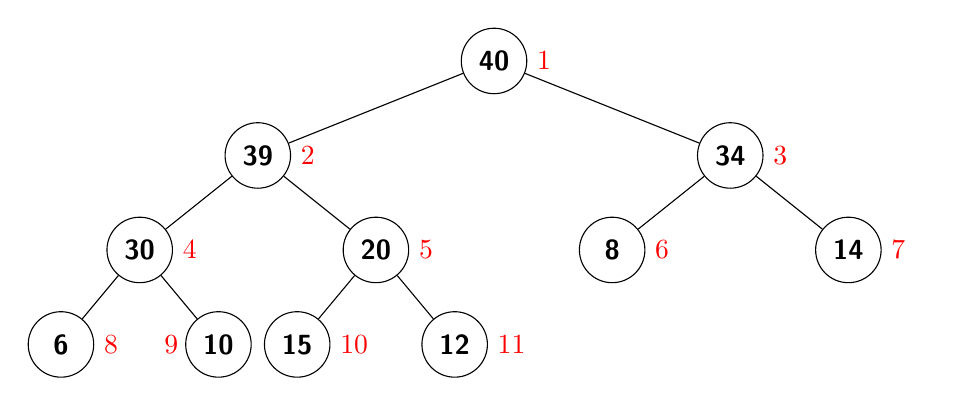
\begin{tikzpicture}[level/.style={sibling distance = 6cm/#1,
  level distance = 1.2cm}]
\node (n40) [bst] {40}
    child {node (n39) [bst] {39}
        child {node (n30) [bst] {30}
            child {node (n6) [bst] {6}}
            child {node (n10) [bst] {10}}
        }
        child {node (n20) [bst] {20}
            child {node (n15) [bst] {15}}
            child {node (n12) [bst] {12}}
        }
    }
    child { node (n34) [bst] {34}
        child{node (n8) [bst] {8}}
        child{node (n14) [bst] {14}}
    }
;
\node [right, txt] at (n40.east) {1};
\node [right, txt] at (n39.east) {2};
\node [right, txt] at (n34.east) {3};
\node [right, txt] at (n30.east) {4};
\node [right, txt] at (n20.east) {5};
\node [right, txt] at (n8.east) {6};
\node [right, txt] at (n14.east) {7};
\node [right, txt] at (n6.east) {8};
\node [txt] at (n10.west) {9};
\node [right, txt] at (n15.east) {10};
\node [right, txt] at (n12.east) {11};
\end{tikzpicture}
\end{document}
